\documentclass[fleqn,11pt]{article}
\usepackage[top=3cm,bottom=3cm,left=3cm,right=3cm,headsep=10pt,a4paper]{geometry} % Page margins

\usepackage{graphicx} % Required for including pictures
\graphicspath{{Pictures/}} % Specifies the directory where pictures are stored

\usepackage{tikz} % Required for drawing custom shapes
\usepackage{dsfont}
\usepackage{enumitem} % Customize lists
\setlist{nolistsep} % Reduce spacing between bullet points and numbered lists

\usepackage{booktabs} % Required for nicer horizontal rules in tables
\usepackage{xcolor} % Required for specifying colors by name
\definecolor{ocre}{RGB}{243,102,25} % Define the orange color used for highlighting throughout the book
\usepackage{microtype} % Slightly tweak font spacing for aesthetics
%\usepackage[utf8]{inputenc} % Required for including letters with accents
%\usepackage[T1]{fontenc} % Use 8-bit encoding that has 256 glyphs

\usepackage{calc} % For simpler calculation - used for spacing the index letter headings correctly
\usepackage{makeidx} % Required to make an index
\makeindex % Tells LaTeX to create the files required for indexing
\usepackage[many]{tcolorbox}
\usepackage{listings}
\usepackage{smartdiagram}
\usetikzlibrary{shadows, arrows, decorations.pathmorphing, fadings, shapes.arrows, positioning, calc, shapes, fit, matrix}
\usepackage{polyglossia}
\usepackage{caption}
\usepackage{subcaption}

\definecolor{lightblue}{RGB}{0,200,255} 
\definecolor{paper}{RGB}{239,227,157}

\pgfdeclarelayer{background}
\pgfdeclarelayer{foreground}
\pgfsetlayers{background,main,foreground}

\lstset{%
  basicstyle=\footnotesize,
  frame=single,
  keywordstyle=\color{blue},
  language=C++,
  commentstyle=\color{red},
  stringstyle=\color{brown},
  keepspaces=true,
  showspaces=false,
  tabsize=2
}

\title{Programmation parallèle}
\author{Juvigny Xavier}
\date{Février 2017}

\newtheorem{prop}{Propriétés }
\newtheorem{remark}{Remarque }

\begin{document}
\maketitle
\tableofcontents

\section{Introduction}

\subsection{Qu'est-ce la programmation parallèle}

La programmation parallèle consiste à concevoir et mettre en œuvre des algorithmes permettant de traiter plusieurs données simultanément dans le but de réduire de restitution par rapport à un algorithme séquentiel effectuant le même traitement sur ces mêmes données, l'algorithme employé ou l'ordre des opérations effectuées pouvant différer. 

Le besoin pour certaines applications de répondre en temps réel ou contraint sur des données de plus en plus complexes ou volumineuses, ou le souhait del'industriel de vouloir réduire le coût d'exécution de l'application, associés à des limites de l'électronique motive l'utilisation de la programmation parallèle. 

\subsection{Quelques cas d'applications nécessitant un traitement intensif des données}
\
\paragraph{Simulation numérique }

De tout temps, la simulation numérique a été consommatrice de mémoire vive et de temps CPU. 

\paragraph{Contrôle-Commande}

Le contrôle-commande permet à l'aide de capteurs permettant de mesurer des paramètres physiques de contrôler et commander à l'aide d'un logiciel un processus physique, par exemple contrôler le processus de fission se développant dans un réacteur nucléaire. 

Ces logiciels sont contraints au temps réel et le nombre de capteurs et par conséquence de paramètres augmente avec le progrès de la technologie.

Par exemple, le contrôle-commande d'un moteur à combustion est devenu de plus en plus complexe au furet à mesure des besoins en rendement, consommation et pollution. En effet, en plus de fournir une puissance mécanique en fonction de l'appui sur la pédale de l'accélérateur,  il est nécessaire d'avoir une optimisation de la consommation du véhicule en contrôlant les différents paramètres de la combustion : pression air, température, mélange,  allumagr, etc. L'ensemble de ces paramètres moteur est géré par un calculateur spécifique. Actuellement,  un véhicule possède de nombreux calculateurs dédiés à des fonctions très diverses : freinage ABS, gestion moteur, éclairage,  climatisation, etc. Ces différents calculateurs communiquent par un bus de terrain afin de partagerles informations et de gérer le véhicule de façon cohérente.

\begin{figure}[h]
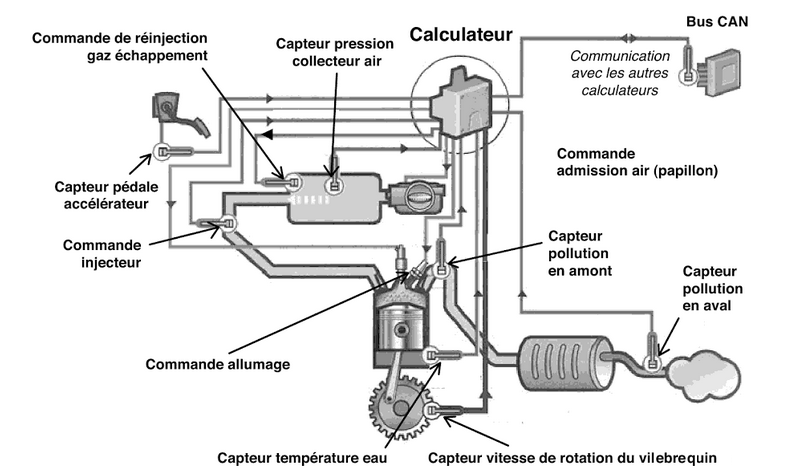
\includegraphics[width=\textwidth]{ControleCommande}
\caption{Représentation schématique de l'application de la commande d'un moteur à combustion.}
\end{figure}

Le contrôle-commande de cette application est faite par l'intermédiaire de \textbf{sept capteurs} ( pédale accélérateur,  température air, pression air, température eau, rotation vilebrequin et deux capteurs de pollution ) et de \textbf{quatre actionneurs} ( injection essence, allumage, admission air, ré-injection gaz échappement ou brûlés ). Le calculateur doit donc en temps réel optimiser le rendement moteur en fonction des sept capteurs et des données reçues des autres calculateurs qui calcul également en parallèle avec leurs propres capteurs et les données qu'ils ont reçu. Si un seul calculateur devzit gérer l'ensemble des capteurs, le calcul d'optimisation serait trop coûteux pour pouvoir le faire en temps réel. Le calcul parallèle distribué mis en place par l'ingénierie automobile à l'aide de calculateurs multiples a permis un contrôle temps réel du rendement moteur. 

\paragraph{Deep learning}

Le deep learning ( apprentissage profond ) est un ensemble de méthodes d'apprentissage automatique fondées sur l'apprentissage de modèles de données. Le deep learning s'applique dans des domaines variés  comme internet ( reconnaissance d'images, traduction automatique, etc.), la médecine  ( détection cellules cancéreuses, détection de drogues, etc. ), la sécurité et la défense  ( détection faciale, surveillance video, \ldots ), l'autonomie des machines ( détection pédestre,  reconnaissance des panneaux de signalisatio, \ldots ).

La plupart des algorithmes de deep learning modélisent un réseau neuronal. Sur un ordinateur séquentiel l'apprentissage dure plus d'une année. La parallélisation sur GPGPU permet de ramener cet apprentissage  à moins de un mois.

Ainsi, Alphago est le premier jeu de go sur ordinateur à avoir battu en Mars 2016 le champion du monde Fan Hui. Basé sur une parallélisation massive sur un cluster de plusieur nœuds de calcul contenant 1202 processeurs et 176 GPGPUs, son apprentissage n'a pris que trois semaines sur seulement cinquante GPGPUs ( contre plusieurs années sur un ordinateur séquentiel ).



\paragraph{Traitement de l'image}

De nos jours, les performances de l'électronique embarquée augmentent regulièrement allant de pair avec une miniaturisation de plus en plus poussée. Il est devenu de ce fait envisageable d'utiliser des capteurs optiques pour la navigation des véhicules autonomes  ( drônes, voiture autonome, etc. ), en calculant des flux optiques entre deux images d'une séquence. 

L'estimation temps réel du flux optique est défini en fonction de la fréquence des images, généralement 25 Hz, voire plus. La résolution des images allant en augmentant, aujourd'hui un système de calcul de flux optique se doit de savoir calculer un flux optique à partir de deux images de $1920\times 1080$ pixels chacune en moins de $\frac{1}{30}$ de secondes soit plus de quatre millions de pixel en un trentième de seconde.

\begin{figure}[h]
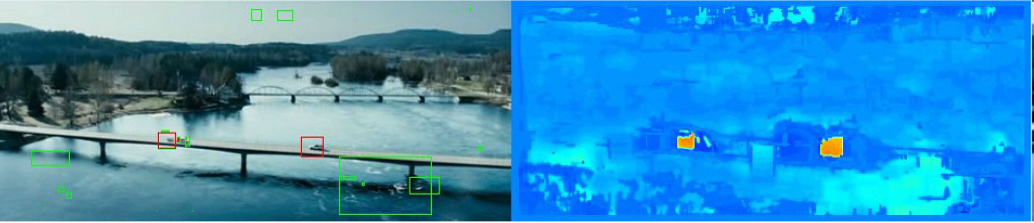
\includegraphics[width=\textwidth]{fluxvideo}
\caption{Détection d'objets en déplacement sur une vidéo aérienne. Sur la gauche, la vidéo d'origine avec des rectangles de détection pour deux niveaux de seuil( vert : faible déplacement, rouge : fort déplacement ). Sur la droite, la norme du flux utilisé pour la détection ( remerciements à Aurélien Plyer pour ses explications sur eFOLKI ).}
\end{figure}

Ainsi, l'ONERA a mis au point un algorithme massivement parallèle sur GPGPU, eFOLKI qui permet de calculer le flux optique enrtre deux images de $1920\times 1080$ pixels chacune en 13ms. Il est donc capable de calculer le flux d'une vidéo à soixante dix images par secondes.

\subsection{La limitation électronique}

Pendant de nombreuses années, des architectures toujours plus complexes et performantes, des gravures toujours plus fines qui permettaient des fréquences toujours plus élevées ont permis aux processeurs de calculer toujours plus vite sans que l'on ait à changer de paradigme de programmation.  

La première difficulté vint avec la mémoire vive dont l'accès aux données ne parvint pas à suivre la fréquence toujours plus haute des processeurs. Qu'importe, on rajouta alors une petite mémoire ultra rapide qui permettait d'accélérer l'accès aux données pour peu qu'on puisse suivant l'algorithme employé lire ou écrire successivement dans une petite région de la mémoire vive. Ces mémoires caches n'ont fait que grossir depuis au fur et à mesure de la montée en puissance des processeurs. 

Durant toutes ces années, les industriels de l'informatique se forcèrent à suivre une "loi" empirique énoncée par \textbf{\textcolor{blue}{Gordon Moore}}, un chercheur de l'entreprise Intel, en 1965 qui  stipule que :
\begin{quote}
Le nombre de transistors dans les microprocesseurs double tous les vingt-quatre mois.
\end{quote}

Depuis quelques années, une seconde difficulté est apparue : la finesse des gravures et la hausse des fréquences induit de plus en plus de chaleur thermique difficile à dissiper. De plus, la finesse des gravures commencent à se heurter à un "mur quantique" matérialisé par l'effet tunnel.

D'autres alternatives au silicium contenu dans les processeurs graphiques sont à l'étude : ordinateur à calcul quantique, ordinateurs neuromorphiques ( composés de neurones ), transistors en graphène, etc. mais aucun n'a encore dépassé le stade de l'expérimentation. 

Actuellement, pour augmenter la puissance de calcul de leurs processeurs, les constructeurs ont donc opté pour augmenter le nombre de c{\oe}urs de calcul sur un même processeur pouvant effectuer des opérations arithmétiques et logiques simultanément. Ainsi,  de nos jours, un processeur "grand public" contiendra de 2 à 8 c{\oe}urs tandis que les processeurs vendus pour les calculateurs auront jusqu'à 72 c{\oe}urs ( le processeur intel Xeon KNL ).

Simultanément, poussés par l'industrie vidéo ludique, les fabricants de cartes graphiques ont accrus la puissance et la souplesse de programmation des cartes graphiques. De GPU ( Graphic Process Unit ), la carte graphique edt devenue GPGPU ( Global Purpose Graphic Process Unit ). L'intérêt des GPGPUs sur les CPUs est de fournir plusieurs milliers d'unités de calcul, d'architectures plus simples que les CPUs ( un GPGPU ne serait pas capable de gérer un système d'exploitation ) pouvant effectuer des calculs en parallèle 
Très vite, on s'aperçut que ce GPGPU pouvait servir de coprocesseur pour accélérer les calculs et les traitements des données. 

Ainsi, dans l'état de l'art actuel, tout programmeur voulant exploiter la puissance des CPUs et des GPGPUs se doit de pouvoir traiter plusieurs données en parallèle sur une machine donnée. On parle alors de \textbf{Programmation parallèle en mémoire partagée}.

Cependant la vitesse d'exécution des programmes avec la montée en puissance des processeurs devient de plus en plus tributaire de l'accès à la mémoire vive. Si la vitesse d'un programme est limitée par l'accès à la mémoire,  on parle alors de programme \textsl{memory bound}, et la vitesse du programme est limitée par la vitesse de traitement du processeur, on parle de programme \textsl{cpu bound}.

Malgré des mémoires caches et des mémoires rapides ( comme la mémoire cache mais gérée entièrement par le programmeur )  toujours plus grandes ( Le KNL d'Intel possède 16Go de mémoire rapide sur son chipset ), permettant si elles sont bien exploitées d'accélérer l'accès à la mémoire, on se retrouve rapidement limité par l'accès mémoire d'autant que le nombre de cœur de calcul est grand.

Il faut donc pouvoir utiliser des unités de calcul ayant chacun sa propre mémoire vive pour encore avoir espoir d'accélérer la vitesse de traitement des données, chaque unité étant alors reliée par un réseau éthernet rapide : On parle alors de cluster et de \textbf{programmation parallèle à mémoire distribuée}.

\section{Architecture des calculateurs parallèles}

Comme nous avons pu voir dans la section précédente, les calculateurs parallèles se déclinent sous plusieurs formes ayant chacun leurs caractéristiques propres. Nous allons classer ces différentes architectures selon les contraintes qu'elles imposent sur la programmation. 

\subsection{Taxonomie de Flynn}

La taxonomie de Flynn est une classification des architectures d'ordinateur, proposée par Michael Flynn en 1966.Les quatre catégories définies par Flynn sont classées selon le type d'organisation d'accès aux données et aux instructions.

Ces quatre catégories sont : 
\begin{enumerate}
\item \textbf{SISD} ( {\bf S}imple {\bf I}nstruction {\bf S}imple {\bf D}ata ) : L'ordinateur n'exécute qu'une seule instruction à la fois qu'il applique que sur une donnée unique. C'est une architecture séquentielle excluant tout parallélisme, dont la programmation n'impose rien de particuliers.

\item \textbf{SIMD} ( {\bf S}imple {\bf I}nstruction {\bf M}ultiple {\bf D}ata ) : L'ordinateur n'exécute qu'une seule instruction à la fois mais celle ci est appliquée simultanément à plusieurs données simultanément. On peut voir cette architecture comme une unité de calcul vectorielle : au lieu de traiter des données scalaires, on traite des données vectorielles. Les unités SSE ou AVX des processeurs Intel peuvent être vues comme des unités SIMD. Les GPGPUs de NVIDIA possèdent des unités de calcul regroupées en "warp",  chaque warp fonctionnant comme une unité SIMD. 

Ces unités de calcul SIMD demandent un soin particulier dans la mise en œuvre des algorithmes. Les instructions demandant des sauts conditionnels ( if, boucles conditionnelles, etc. ) peuvent être très pénalisantes sur ce type de machines, dû au système de masques utilisé pour ce type d'instructions. Par exemple, considérons le bout de code suivant :

\begin{lstlisting}[language=C++]
if ( a[i]>= 0 )
  b[i] = c[i];
else
  b[i] = -d[i];
\end{lstlisting}

Une machine SIMD traitera simultanément plusieurs indices i simultanément, mais en appliquant exactement  la même instruction élémentaire.  Pour l'exemple ci-dessus, elle ne pourra pas appliquer les deux embranchements simultanément et devra utiliser un système de masque. Elle exécutera donc un code équivalent au code précédent  comme suit :

\begin{lstlisting}[language=C++]
msk[i] = a[i]>=0;// = 1 si vrai, 0 sinon
b[i] = msk[i] * c[i] - (1-msk[i]) * d[i];
\end{lstlisting}

On voit donc sur cet exemple que la machine SIMD est obligée  d'évaluer les deux conditions contrairement à une unité de calcul classique qui évalue l'une ou l'autre condition pour chaque i.

Pour les boucles conditionnelles,  le problème est encore plus crucial. Considérons la boucle suivante qui effectue des itérations simultanées sur plusieurs suites de Mandelbrot 
$z_{n+1}[i]= z^{2}_{n}[i]+c[i]$ jusqu'à détecter une divergence lorsque 
$\left|z_{n}[i]\right| \geq 2$ pour divers $i$ avec $c[i]$ fixé pour chaque i. 

\begin{lstlisting}[language=C++]
const long nIterMax = 65000;
z[i] = 0;
iter[i] = 0;
while ( (abs (z[i] ) < 2) && (iter[i] < nIterMax) )
{
  z[i] = z[i]*z[i]+c[i];
  iter[i] += 1;
}
\end{lstlisting}

Cette suite peut très bien diverger rapidement pour un \texttt{c[i]} donné et converger pour une valeur
de \texttt{c[i]} proche ! Ainsi, certaines unités de calcul devront faire un grand nombre d'itérations
pendant que d'autres en font très peu. Que se passe t'il dans le cas d'unités de calcul SIMD ?

Il est clair que toutes les UCs doivent itérer tant que l'une d'elles calcule une suite qui n'a pas encore divergé, du fait que toutes les UCs doivent exécuter la même instruction simultanément. Et un système de masque permettra aux suites ayant divergé de stagner sur la même valeur. Le code exécuté par des UCs SIMD ressemblera alors au pseudo code C++ suivant :

\begin{lstlisting}[language=C++]
const long nIterMax = 65000;
z[i] = 0;
iter[i] = 0;
msk[i] = true;
while ( find (msk,true) ) // Tant qu'un des masques d'une UC est vrai
{
  z[i] = msk[i]*(z[i]*z[i]+c[i]) + (1-msk[i])*z[i];
  iter[i] += msk[i];
  msk[i] = (abs (z[i]) < 2) && (iter[i] < nIterMax);
}
\end{lstlisting}

Ainsi, chaque UC devra itérer autant de fois que l'UC itérant le plus, consommant inutilement de la puissance de calcul.

C'est pour ces raisons que les machines massivement SIMD telle que la connection machine dans les années 1980 ( qu'on peut voir à la fin du film Jurrasic Park )  ont été peu à peu abandonnées au début des années 1990. Néanmoins l'architecture SIMD est reapparue sous forme de petites unités de calcul avec les GPGPUs et les registres vectoriels d'Intel.

\item \textbf{MISD} ({\bf M}ultiple {\bf I}nstruction {\bf S}imple {\bf D}ata) : Dans ce type de calculateur, une seule donnée est lue à la fois mais plusieurs instructions opèrent simultanément un traitement dessus. Cela peut sembler paradoxal mais recouvre en fait un type très ordinaire de micro-parallélisme dans les microprocesseurs modernes : les architectures pipelines associées aux registres vectoriels. 

\begin{figure}[h]
\begin{lstlisting}[language=C++]
for ( int i = 1; i <= 4; ++i )
  r[i] = a[i] + b[i];
\end{lstlisting}

\begin{tikzpicture}
\matrix (timeline) [matrix of nodes,nodes={draw,text width=15mm}]
{
  Lire $a_{1}$ & Lire $a_{2}$ & Lire $a_{3}$ & Lire $a_{4}$ &              &              & \\
               & Lire $b_{1}$ & Lire $b_{2}$ & Lire $b_{3}$ & Lire $b_{4}$ &              & \\
               &              &$a_{1}+b_{1}$ &$a_{2}+b_{2}$ &$a_{3}+b_{3}$ &$a_{4}+b_{4}$ & \\
| [draw=none] | \phantom{a} & & & Écrire $r_{1}$ &Écrire $r_{2}$&Écrire $r_{3}$&Écrire $r_{4}$ \\
};
\node[below left=1em of timeline-4-1.south west]  (a00) {};
\node[below right=1em of timeline-4-7.south east] (a01) {};
\node[above left=1em of timeline-1-1.north west]  (a10) {};
\draw[thick,red,->,>=latex] (a00) to node[below]{Temps} (a01);
\draw[thick,blue,->,>=latex] (a00) to node[above,sloped]{Instructions} (a10);
\end{tikzpicture}
\caption{Principe d'une architecture pipeline}\label{fig:pipeline}
\end{figure} 

Sur la figure (\ref{fig:pipeline}), on remplit les registres vectoriels $a$ et $b$ petit à petit, et dans le même instant, on effectue une addition sur les parties de $a$ et $b$ déjà remplies.

\item \textbf{MIMD} ( {\bf M}ultiple {\bf I}nstruction {\bf M}ultiple {\bf D}ata )

Cette architecture permet de lire/écrire plusieurs données et d'effectuer des traitements différents sur ces données simultanément. Les processeurs multi cœurs des machines actuelles sont des unités MIMD.

\end{enumerate}

\begin{figure}[h]
\begin{center}
\begin{tikzpicture}
\node[fill=cyan, draw, rotate=90] (Data) {Données};
\node[fill=orange, draw, circle, right=10ex of Data.south ] (UC) {UC};
\node[fill=yellow, draw, above=10ex of UC.north] (I) {Instructions};
\draw[-latex,red] (Data) -- (UC);
\draw[-latex, blue] (I) -- (UC);
\node[below=5ex of UC.south] {Architecture SISD};
\end{tikzpicture}
\qquad
\begin{tikzpicture}
\node[fill=cyan, draw, rotate=90] (Data) {Données};
\node[right=10ex of Data.south ] (UC0) {\phantom{\LARGE UC}};
\node[fill= orange, circle,draw,left=2em of UC0.north, inner sep=1pt] (UC1) {\scriptsize UC};
\node[fill= orange, circle,draw,right=2em of UC0.north, inner sep=1pt] (UC2) {\scriptsize UC};
\node[fill= orange, circle,draw,left=2em of UC0.south, inner sep=1pt] (UC3) {\scriptsize UC};
\node[fill= orange, circle,draw,right=2em of UC0.south, inner sep=1pt] (UC4) {\scriptsize UC};
\node[fill=yellow, draw, above=10ex of UC0.north] (I) {Instructions};
\draw[-latex,red] (Data.340) -- (UC2.135);
\draw[-latex,red] (Data.300) -- (UC1);
\draw[-latex,red] (Data.200) -- (UC4.225);
\draw[-latex,red] (Data.240) -- (UC3);
\draw[blue] (I) -- (UC0.center);
\draw[-latex, blue] (UC0.center) -- (UC1.east);
\draw[-latex, blue] (UC0.center) -- (UC3.east);
\draw[-latex, blue] (UC0.center) -- (UC2.west);
\draw[-latex, blue] (UC0.center) -- (UC4.west);
\node[below=5ex of UC.south] {Architecture SIMD};
\end{tikzpicture}

\begin{tikzpicture}
\node[fill=cyan, draw, rotate=90] (Data) {Données};
\node[right=10ex of Data.south ] (UC0) {\phantom{\LARGE UC}};
\node[fill= orange, circle,draw,left=2em of UC0.north, inner sep=1pt] (UC1) {\scriptsize UC};
\node[fill= orange, circle,draw,right=2em of UC0.north, inner sep=1pt] (UC2) {\scriptsize UC};
\node[fill= orange, circle,draw,left=2em of UC0.south, inner sep=1pt] (UC3) {\scriptsize UC};
\node[fill= orange, circle,draw,right=2em of UC0.south, inner sep=1pt] (UC4) {\scriptsize UC};
\node[fill=yellow, draw, above=10ex of UC0.north] (I) {Instructions};
\draw[-latex,blue] (I.340) to[bend left] (UC4.45);
\draw[-latex,blue] (I.300) -- (UC2);
\draw[-latex,blue] (I.200) to[bend right] (UC3.135);
\draw[-latex,blue] (I.240) -- (UC1);
\draw[red] (Data) -- (UC0.center);
\draw[-latex, red] (UC0.center) -- (UC1.east);
\draw[-latex, red] (UC0.center) -- (UC3.east);
\draw[-latex, red] (UC0.center) -- (UC2.west);
\draw[-latex, red] (UC0.center) -- (UC4.west);
\node[below=5ex of UC.south] {Architecture MISD};
\end{tikzpicture}
\qquad
\begin{tikzpicture}
\node[fill=cyan, draw, rotate=90] (Data) {Données};
\node[right=10ex of Data.south ] (UC0) {\phantom{\LARGE UC}};
\node[fill= orange, circle,draw,left=2em of UC0.north, inner sep=1pt] (UC1) {\scriptsize UC};
\node[fill= orange, circle,draw,right=2em of UC0.north, inner sep=1pt] (UC2) {\scriptsize UC};
\node[fill= orange, circle,draw,left=2em of UC0.south, inner sep=1pt] (UC3) {\scriptsize UC};
\node[fill= orange, circle,draw,right=2em of UC0.south, inner sep=1pt] (UC4) {\scriptsize UC};
\node[fill=yellow, draw, above=10ex of UC0.north] (I) {Instructions};
\draw[-latex,blue] (I.340) to[bend left] (UC4.45);
\draw[-latex,blue] (I.300) -- (UC2);
\draw[-latex,blue] (I.200) to[bend right] (UC3.135);
\draw[-latex,blue] (I.240) -- (UC1);
\draw[-latex,red] (Data.340) -- (UC2.135);
\draw[-latex,red] (Data.300) -- (UC1);
\draw[-latex,red] (Data.200) -- (UC4.225);
\draw[-latex,red] (Data.240) -- (UC3);
\node[below=5ex of UC.south] {Architecture MIMD};
\end{tikzpicture}

\begin{tikzpicture}
\node[fill= orange, circle,draw, inner sep=1pt] (UC) {UC};
\node[right=1em of UC.east] {Unité de calcul};
\end{tikzpicture}
\end{center}
\caption{Taxonomie de Flynn}
\end{figure}

\subsection{Mémoire partagée et mémoire distribuée}

La mémoire vive est un composant limitant l'efficacité du traitement des données dans un calculateur. 

\begin{figure}
\begin{center}
\begin{tikzpicture}
\draw[->,>=latex] (0,0) -- (10,0);
\draw[->,>=latex] (0,0) -- (0,10);
\foreach \x/\xtext in {0/1980,2/1985, 4/1990, 6/1995, 8/2000, 10/2005} {
  \draw (\x,0) -- (\x,-1mm) node[below]{\xtext};
}
\foreach \y/\ytext in {0/1, 2/10, 4/100, 6/10^3, 8/10^4, 10/10^5} {
  \draw[dashed,ocre] (-1mm, \y) node[black,left]{$\ytext$} -- (10, \y);
}
\draw[blue] (0,0) -- (2.5,1.6) -- node[above,black]{CPU} (10,8.25);
\draw[red] (0,0) -- node[black,above]{Mémoire} (10,1.8);
\node[black] at (5,9) {Performances relatives à celles de 1980};
\end{tikzpicture}
\end{center}
\caption{Comparaison de l'évolution des unités de calcul et de la mémoire vive}
\label{fig:compucram}
\end{figure}

Comme on peut le voir sur la figure (\ref {fig:compucram}), l'évolution de l'efficacité des mémoires vives est bien plus lente que celle des unités de calculs. C'est pour cela que 
les calculateurs actuels offrent deux types de mémoire:

\begin{itemize}
\item \textbf{La mémoire partagée} : Les différentes unités de calcul de calcul partagent une même mémoire vive centrale au travers d'un bus mémoire. Cependant, la mémoire vive est d'un accès lent par rapport au traitement dont sont capables les processeurs actuels. Plusieurs techniques existent pour accélérer l'accès aux données :
  \begin{itemize}
  \item \textsl{La mémoire vive entrelacée} : Une mémoire entrelacée à $n$ voies de largeur $w$ est constituée de $n$ blocs mémoires. Le bloc numéroté $i$, avec $i\in \left[0, n-1\right]$ contient toutes les cellules dont les adresses sont égales à $w\times ( n \times a + i ) +  k $ avec $k\in \left[0,w-1\right]$ et $a\in \mathds{N}$. De cette manière, deux mots de largeur $w$ rangés consécutivement sont stockés dans deux blocs différents. Cette organisation permet de réduire  le temps d'accès à la mémoire lors de la lecture ou de l'écriture par groupe de mots.

Supposons qu'une unité de calcul de cycle $\delta t$ dont la mémoire principale possède un temps d'accès de $\delta ta$  après réception d'une requête, veuille lire un ensemble de $N$ valeurs de taille $w$ par valeur, rangées de façon contigüe dans un tableau. Dans une mémoire non entrelacée, cette opération demande un temps $\Delta t_{1} = N.\delta ta$

\begin{figure}[h]
\begin{center}
\begin{tikzpicture}
\draw[->,>=latex] (0,0) -- (10,0) node[below]{cycle};
\foreach \x in {0,1,...,9} {
  \draw (\x,1mm) -- (\x,-1mm) node[below] {$\x\strut$};
}
\draw[->,>=latex,blue] (0,1.5cm) node[above,black] {Requêtes} -- (0,2mm);
\draw[->,>=latex,red] (4,1.5cm) -- (4,2mm);
\draw[->,>=latex,violet] (8,1.5cm) -- (8,2mm);

\draw[->,>=latex,blue] (4,-4ex) -- (4,-1.5cm) node[below,black]{Données};
\draw[->,>=latex,red] (8,-4ex) -- (8,-1.5cm);
\end{tikzpicture}
\end{center}
\caption{Accès à une mémoire non entrelacée}
\end{figure}

Dans une mémoire entrelacée à $n$ voies, telle que $\delta ta \leq n.\delta t$, la première requête est transmise au bloc $i$ de la mémoire. Au cycle d'horloge suivant, la seconde requête est transmise au bloc $i+1$, et ainsi de suite. Chacune des $n$ premières requêtes est ainsi transmise à un bloc différent. Ces blocs fonctionnent soit en parallèle  ( il possible de faire des requêtes simultanées sur des blocs différents )  soit en pipeline ( une requête par cycle d'horloge sur des blocs différents ). À l'instant $\delta ta$ après la première requête, la première donnée est disponible. La deuxième donnée est disponible un cycle $\delta t$ plus tard et ainsi de suite comme illustré sur la figure (\ref{fig:entrelacee}).

\begin{figure}[h]
\begin{center}
\begin{tikzpicture}
\draw[->,>=latex] (0,0) -- (10,0) node[below]{cycle};
\foreach \x in {0,1,...,9} {
  \draw (\x,1mm) -- (\x,-1mm) node[below] {$\x\strut$};
}
\draw[->,>=latex,blue] (0,1.5cm) node[above,black] {Requêtes} -- (0,2mm);
\foreach \x/\col in {1/red,2/violet,3/ocre,4/blue,5/red,6/violet,7/ocre,8/blue,9/red}{
  \draw[->,>=latex,\col] (\x,1.5cm) -- (\x,2mm);
}
\draw[->,>=latex,blue] (4,-4ex) -- (4,-1.5cm) node[below,black] {Données};
\foreach \x/\col in {5/red,6/violet,7/ocre,8/blue,9/red}{
  \draw[->,>=latex,\col] (\x,-4ex) -- (\x,-1.5cm);
}
\end{tikzpicture}
\end{center}
\label{fig:entrelacee}
\caption{Accès à une mémoire entrelacée à quatre voies}
\end{figure}

Les données suivantes pourront être récupérées à chaque cycle. Il faut donc un temps $\Delta t_{2} = \delta ta + N.\delta t $ pour lire $N$ valeurs et attendre un temps  $\delta ta$ sans accéder à aucune donnée.

Ce type de mémoire, dont le coût dépend du nombre de voies et coûte bien plus chère que la mémoire non entrelacée est principalement utilisée sur les GPGPUs et est associée avec de la mémoire cache. 

\item \textsl{La hiérarchie de mémoire cache} : 
La mémoire cache sur les unités séquentielles permettent, lorsqu'elles sont bien employées, c'est à dire lorsque la mise en œuvre de l'algorithme satisfait à un accès local temporel et spatial des variables  ( on essaie de reutiliser successivement le plus possible un même petit ensemble de données ) d'accélérer de façon significative le traitement des données par une unité de calcul. Néanmoins, sur un calculateur parallèle, la mémoire cache obéit également à d'autres contraintes du fait du partage de certains niveaux de cache et de la mémoire vive entre les différentes unités de calcul. 

\begin{figure}[h]
\begin{center}
\begin{tikzpicture}
\node[rounded corners, drop shadow,draw,fill=blue!50!white,text height=1.5ex] (M) {Mémoire vive};
\node[rounded corners, drop shadow,draw,fill=green!50!white, right= 6em of M.east, text height=1.5ex] (E) {Entrée - Sortie};
\node[below=4ex of M.south] (B) {};
\node[below=4ex of E.south] (Be) {};
\node[below=4ex of M.south west] (B0) {};
\foreach \x/\n in {1/B0,2/B1,3/B2,4/B3} {
  \node[right=4em of \n.east] (B\x) {};
  \node[below=2ex of B\x.south,draw,text width=3em] (C\x) {Cache};
  \node[below=1ex of C\x.south,draw,text width=3em] (P\x) {UC};
  \draw[ocre,thick] ($(C\x.north west)+(-0.1,0.1)$) rectangle ($(P\x.south east)+(0.1,-0.1)$);
  \draw[blue] (B\x.center) -- (C\x);
}
\node[right=4ex of B4.east] (B5) {};
\draw[blue] (B0.west) -- (B5.east);
\draw[blue] (M) -- (B.center);
\draw[blue] (E) -- (Be.center);
\node[above= 1 ex of B2.north] {Bus de données};
\end{tikzpicture}
\end{center}
\caption{Organisation de la mémoire cache dans un calculateur multi--processeur}
\label{fig:cachemultiproc}
\end{figure}

Dans le cas d'une machine multiprocesseurs ( voir figure (\ref{fig:cachemultiproc} ), il faut assurer la cohérence des données entre mémoires caches :
\begin{itemize}
\item Seul cette mémoire cache contient la donnée. Elle est donc valide et aucune synchronisation n'est nécessaire avec la mémoire vive;
\item La donnée est partagée avec d'autres caches. Il faut donc vérifier à chaque accès si elle n'a pas été modifiée par d'autres processeurs et la marquer dzns ce cas comme invalide.
\item La valeur a été modifiée dans le cache et la valeur en mémoire vive n'est plus à jour. Il faudra donc mettre à jour la mémoire vive si d'autres processeurs veulent lire la valeur;
\item La valeur dans la mémoire cache est invalide. La prochaine lecture de cette valeur déclenchera une lecture en mémoire vive. 
\end{itemize}

\begin{figure}[h]
\begin{center}
\begin{tikzpicture}
\node[rounded corners, drop shadow,draw,fill=blue!50!white,text height=1.5ex] (M) {Mémoire vive};
\node[rounded corners, drop shadow,draw,fill=green!50!white, right= 6em of M.east, text height=1.5ex] (E) {Entrée - Sortie};
\node[below=4ex of M.south] (B) {};
\node[below=4ex of E.south] (Be) {};
\node[below=4ex of M.south west] (B0) {};
\node[right=6em of B.east] (B1) {};
\node[right=14em of B1.east] (Br) {};
\node[below=7ex of B1.south,text width = 16em,fill=cyan!25,draw,text centered] (L3) {Cache L3};
\node[below=2ex of L3.south] (BL3) {};
\node[left=3em of BL3.west,draw,text width = 4em,fill=cyan!40,text centered] (L21) {\small Cache L2};
\node[right=3em of BL3.east,draw,text width = 4em,fill=cyan!40, text centered] (L22) {\small Cache L2};

\node[below=1.5em of L21.south] (BL21) {};
\node[left=0.3em of BL21.west,draw,text width = 3.5em,fill=cyan!55, text centered] (L111) {\scriptsize Cache L1};
\node[below=1ex of L111.south,draw,text width = 3.5em,fill=red!55, text centered] (U111) {\scriptsize UC};
\draw[blue,thick] ($(U111.south west)+(-0.1,-0.1)$) rectangle ($(L111.north east)+(0.1,0.1)$);
\node[right=0.3em of BL21.east,draw,text width = 3.5em,fill=cyan!55, text centered] (L112) {\scriptsize Cache L1};
\node[below=1ex of L112.south,draw,text width = 3.5em,fill=red!55, text centered] (U112) {\scriptsize UC};
\draw[blue,thick] ($(U112.south west)+(-0.1,-0.1)$) rectangle ($(L112.north east)+(0.1,0.1)$);

\node[below=1.5em of L22.south] (BL22) {};
\node[left=0.3em of BL22.west,draw,text width = 3.5em,fill=cyan!55, text centered] (L121) {\scriptsize Cache L1};
\node[below=1ex of L121.south,draw,text width = 3.5em,fill=red!55, text centered] (U121) {\scriptsize UC};
\draw[blue,thick] ($(U121.south west)+(-0.1,-0.1)$) rectangle ($(L121.north east)+(0.1,0.1)$);
\node[right=0.3em of BL22.east,draw,text width = 3.5em,fill=cyan!55, text centered] (L122) {\scriptsize Cache L1};
\node[below=1ex of L122.south,draw,text width = 3.5em,fill=red!55, text centered] (U122) {\scriptsize UC};
\draw[blue,thick] ($(U122.south west)+(-0.1,-0.1)$) rectangle ($(L122.north east)+(0.1,0.1)$);

\draw[ocre,thick] ($(U111.south west)+(-0.2,-0.2)$) rectangle ($(L21.north -| L112.east)+(0.2,0.1)$);
\draw[ocre,thick] ($(U121.south west)+(-0.2,-0.2)$) rectangle ($(L22.north -| L122.east)+(0.2,0.1)$);

\draw[ocre!50!blue,thick] ($(U111.south west)+(-0.3,-0.3)$) rectangle ($(L3.north -| L122.east)+(0.3,0.1)$);

\draw[blue] (B0.west) -- (Br.east);
\draw[blue] (M) -- (B.center);
\draw[blue] (E) -- (Be.center);
\draw[blue] (B1.center) -- (L3);
\draw[blue!75] (L3) -- (BL3.center);
\draw[blue!75] (BL3.center) -- (L21);
\draw[blue!75] (BL3.center) -- (L22);
\draw[blue!50] (L21) -- (BL21.center);
\draw[blue!50] (BL21.center) -- (L111);
\draw[blue!50] (BL21.center) -- (L112);

\draw[blue!50] (L22) -- (BL22.center);
\draw[blue!50] (BL22.center) -- (L121);
\draw[blue!50] (BL22.center) -- (L122);
\draw[orange,dashed] (L21.south east) -- node[below] {\scriptsize \textcolor{black}{Bus}} (L22.south west);
\end{tikzpicture}
\end{center}
\caption{Organisation de la mémoire cache dans un calculateur multi--cœur}
\label{fig:cachemulticoeur}
\end{figure}

Dans le cas d'une machine multi--cœurs, plusieurs unités de calcul partagent les mêmes niveaux de cache ( voir la figure (\ref{fig:cachemulticoeur}) ) afin d'éviter de passer par la mémoire vive pour s'assurer de la cohérence des données en mémoire cache. De plus, afin d'éviter de remonter d'un niveau de cache, les multi--cœurs récents possèdent des bus reliant les mémoires caches d'un même niveau. Lors de l'optimisation d'un code sur une machine multi--cœurs, il est important d'avoir cette organisation des mémoires caches en tête afin d'organiser les threads et les données de sorte à ce qu'un minimum de données transitent par les bus reliant les mémoires caches. Cela impose donc les mêmes contraintes qu'une machine NUMA ( Non Uniform Memory Access ) que nous allons voir plus loin.

\end{itemize}

\item \textbf{La mémoire distribuée}

L'efficacité d'une machine multi--cœurs dépend de l'organisation de sa mémoire qui, pour être efficace demande une architecture complexe et onéreuse dont le coût est sur-linéaire au nombre de cœurs. Afin d'obtenir un calculateur performant sans être prohibitif, chaque unité de calcul ( en général multi--cœurs ) possède  sa propre mémoire vive. Un ensemble unité de calcul multi cœur et mémoire vive s'appelle un \textbf{nœud de calcul} sur les machines distribuées. 

 Ces différentes unités de calcul échangent des données au travers d'un bus spécialisé ou  plus souvent au travers d'un réseau de type Gigabit. On parle alors d'un calculateur \textsl{à mémoire distribuée}. Ce type de calculateur a un coût de fabrication linéaire en fonction du nombre d'unités de calcul sur le réseau du calculateur. 

La programmation de ces calculateurs demande une mise en œuvre spécifique et fréquemment des algorithmes spécifiques permettant d'exploiter efficacement la capacité de calcul de la machine.

Ce type de calculateur permet d'exploiter simultanément plusieurs dizaines de milliers d'unités de calcul. Cependant, la lenteur relative des réseaux ou des bus ainsi que le ''degré de parallélisme'' de l'algorithme employé limitent la rapidité de traitement des donnees

\begin{figure}[h]
\begin{center}
\begin{tikzpicture}
\node[draw,fill=blue!50!white, drop shadow, rounded corners] (Ram1) {Mémoire vive};
\node[below=2ex of Ram1.south] (B1) {};
\node[left=1em of B1.west,draw,fill=red!55] (U1) {UC};
\node[right=1em of B1.east,draw,fill=red!55] (U2) {UC};
\draw[blue] (Ram1) -- (B1.center);
\draw[blue] (B1.center) -- (U1);
\draw[blue] (B1.center) -- (U2);

\node[draw,fill=blue!50!white, drop shadow, rounded corners,left=10em of Ram1.east] (Ram2) {Mémoire vive};
\node[below=2ex of Ram2.south] (B2) {};
\node[left=1em of B2.west,draw,fill=red!55] (U3) {UC};
\node[right=1em of B2.east,draw,fill=red!55] (U4) {UC};
\draw[blue] (Ram2) -- (B2.center);
\draw[blue] (B2.center) -- (U3);
\draw[blue] (B2.center) -- (U4);

\node[draw,fill=blue!50!white, drop shadow, rounded corners,left=10em of Ram2.east] (Ram3) {Mémoire vive};
\node[below=2ex of Ram3.south] (B3) {};
\node[left=1em of B3.west,draw,fill=red!55] (U5) {UC};
\node[right=1em of B3.east,draw,fill=red!55] (U6) {UC};
\draw[blue] (Ram3) -- (B3.center);
\draw[blue] (B3.center) -- (U5);
\draw[blue] (B3.center) -- (U6);

\node[above=2ex of Ram1.north] (R1) {};
\node[above=2ex of Ram2.north] (R2) {};
\node[above=2ex of Ram3.north] (R3) {};
\node[right=1em of R1.east] (R0){};
\node[left=1em of R3.west] (R4) {};
\draw[thick,red] (R0.east) -- (R1.center) -- (R2.center) node[above] {Réseau}-- (R3.center) -- (R4.west);
\draw[thick,red] (Ram1) -- (R1.center);
\draw[thick,red] (Ram2) -- (R2.center);
\draw[thick,red] (Ram3) -- (R3.center);
\end{tikzpicture}
\end{center}
\caption{Architecture calculateur à mémoire distribuée}
\label{fig:archmemdistrib}
\end{figure}

Les réseaux connectant les différentes unités de calcul offrent des topologies variées. Il peut être important d'avoir en tête la topologie du calculateur employé. En effet, les données échangées via le réseau transiteront selon la topologie du réseau via d'autres unités de calcul, ce qui ralentira les échanges de données en fonctiin du nombre d'unités de calcul intermédiaires par lesquelles les données transiteront. Pour calculer le nombre maximal de nœuds intermédiaires,  on définit pour un réseau la distance entre deux nœuds et son diamètre :

%\begin{theorem}
On appelle \textbf{distance entre deux nœuds} sur un réseau donné le minimum de nœuds
intermédiaires par lesquels doivent transiter des données echangées entre les deux
nœuds.
%\end{theorem}

On appelle \textbf{diamétre d'un réseau} la distance maximale entre
deux nœuds du réseau. 

Pour la commodité de l'exposé, et en adéquation avec la vue programmeur
fournie par les bibliothèques de calcul parallèle distribuée, on numérote
chacun des $N$ nœuds de calcul de façon unique à l'aide d'un nombre entre
0 et $N-1$.

\begin{itemize}
\item \textbf{Topologie linéaire}

Les $N$ nœuds de calcul sont reliés de sorte qu'on peut trouver une numérotation
des nœuds de calcul tel qu'un nœud $i$ est seulement lié directement au
nœud $i-1$ ( si $ i > 0$ ) et au nœud $i+1$ ( si $i < N-1$ ).

\begin{figure}
\begin{center}
\begin{tikzpicture}
\node[text width=2.2em,draw,fill=yellow,drop shadow, text centered] (N0) {\small Nœud 0};
\node[below= 2ex of N0.south] (C0) {};
\draw[thick,red] (N0) -- (C0.center);
\foreach \x/\p in {1/0,2/1,3/2} {
\node[text width=2.2em, right=2em of N\p.east,draw,fill=yellow,drop shadow, text centered] (N\x) {\small Nœud \x};
\node[below= 2ex of N\x.south] (C\x) {};
\draw[thick,red] (N\x) -- (C\x.center);
}
\node[left=2em of C0.west] (Cb) {};
\node[right=2em of C3.east] (Ce) {};
\draw[thick,red] (Cb) -- (Ce);
\end{tikzpicture}
\end{center}
\label{fig:reslin}
\caption{Réseau Linéaire}
\end{figure}

Le diamètre de ce réseau est $N-1$.

\item \textbf{Topologie anneau}

La topologie de ce réseau est similaire à celui d'un réseau linéaire.
Seule différence notable, le nœud 0 est relié au nœud $N-1$.

\begin{figure}
\begin{center}
\begin{tikzpicture}
\node[text width=2.2em,draw,fill=yellow,drop shadow, text centered] (N0) {\small Nœud 0};
\node[below= 2ex of N0.south] (C0) {};
\draw[thick,red] (N0) -- (C0.center);
\foreach \x/\p in {1/0,2/1,3/2} {
\node[text width=2.2em, right=2em of N\p.east,draw,fill=yellow,drop shadow, text centered] (N\x) {\small Nœud \x};
\node[below= 2ex of N\x.south] (C\x) {};
\draw[thick,red] (N\x) -- (C\x.center);
}
\node[above=1em of N0.north] (L) {};
\node[above=1em of N3.north] (R) {};
\draw[thick,red] (N0) -- (L.center) -| (R.center) -- (N3);
\draw[thick,red] (C0.center) -- (C3.center);
\end{tikzpicture}
\end{center}
\label{fig:resanneau}
\caption{Réseau en anneau}
\end{figure}

Le réseau étant bidirectionnel, le diamètre de ce réseau est $\frac{N}{2}$ si le nombre
de nœud $N$ est pair, $\frac{N-1}{2}$ sinon.

\item \textbf{Topologie grille}

Le réseau connectant les $N=W\times H$ nœuds est topologiquement équivalent à
une grille de $W\times H$ nœuds.

\begin{figure}[h]
\begin{center}
\begin{tikzpicture}
\node (O0) {};
\foreach \i in {1,2,3,4}{
  \pgfmathtruncatemacro{\im}{\i-1};
  \node[below=1ex of O\im.south] (O\i) {};
  \foreach \j in {1,2,3} {
    \pgfmathtruncatemacro{\ipj}{\i+(\j-1)*4-1};
    \node[text width=1em, fill=yellow, drop shadow] at (\i cm, \j cm) (Nd\i\j)
    {\scriptsize $N_{\ipj}$};
  }
}
\foreach \i in {1,2,3}{
  \pgfmathtruncatemacro{\ip}{\i+1};
  \foreach \j in {1,2} {
    \pgfmathtruncatemacro{\jp}{\j+1};
    \draw[red,thick] (Nd\i\j) -- (Nd\ip\j);
    \draw[red,thick] (Nd\i\j) -- (Nd\i\jp);
  }
}
\foreach \i in {1,2,3}{
  \pgfmathtruncatemacro{\ip}{\i+1};
    \draw[red,thick] (Nd\i3) -- (Nd\ip3);
}
\foreach \j in {1,2} {
    \pgfmathtruncatemacro{\jp}{\j+1};
    \draw[red,thick] (Nd4\j) -- (Nd4\jp);
  }
\end{tikzpicture}
\end{center}
\caption{Réseau sur grille}
\label{fig:gridnet}
\end{figure}

On voit, en considérant la communication du premier n{\oe}ud avec le dernier
n{\oe}ud que le diamètre d'un réseau sur grille est égal à $W+H-2$.

\item \textbf{Topologie hyper cube}

La topologie hyper cube est une topologie telle que la connection des n{\oe}uds de calcul
est équivalente à celle reliant les sommets d'un hyper cube de dimension $n$.

\begin{figure}[h]
\centering
\begin{subfigure}[c]{0.46\textwidth}
\centering
\begin{tikzpicture}
\node[text width=1em, fill=yellow, drop shadow]  (N0) {\scriptsize $N_{0}$};
\end{tikzpicture}
\caption{$\mathcal{C}_{0}$ : hypercube de dimension 0}\label{fig:HypCub0}
\end{subfigure}
\qquad
\begin{subfigure}[c]{0.46\textwidth}
\centering
\begin{tikzpicture}
\node[text width=1em, fill=yellow, drop shadow]  (N0) {\scriptsize $N_{0}$};
\node[right=2em of N0.east, text width=1em, fill=yellow, drop shadow] (N1) {\scriptsize $N_{1}$};
\draw[thick,red] (N0) -- (N1);
\end{tikzpicture}
\caption{$\mathcal{C}_{1}$ : hypercube de dimension 1}\label{fig:HypCub1}
\end{subfigure}

\begin{subfigure}[c]{0.46\textwidth}
\centering
\begin{tikzpicture}
\node[text width=1em, fill=yellow, drop shadow]  (N0) {\scriptsize $N_{00}$};
\node[right=2em of N0.east, text width=1em, fill=yellow, drop shadow] (N1) {\scriptsize $N_{01}$};
\node[text width=1em, fill=yellow!76!red, drop shadow, above=4ex of N0.north] (N2) {\scriptsize $N_{10}$};
\node[right=2em of N2.east, text width=1em, fill=yellow!76!red, drop shadow] (N3) {\scriptsize $N_{11}$};
\draw[thick,red](N0) -- (N1);
\draw[thick,red](N0) -- (N2);
\draw[thick,red](N2) -- (N3);
\draw[thick,red](N1) -- (N3);
\end{tikzpicture}
\caption{$\mathcal{C}_{2}$ : hypercube de dimension 2}\label{fig:HypCub2}
\end{subfigure}
\qquad
\begin{subfigure}[c]{0.46\textwidth}
\centering
\begin{tikzpicture}
\node[text width=2em, fill=yellow, drop shadow]  (N0) {\scriptsize $N_{000}$};
\node[right=3em of N0.east, text width=2em, fill=yellow, drop shadow] (N1) {\scriptsize $N_{001}$};
\node[text width=2em, fill=yellow!76!red, drop shadow, above=4ex of N0.north] (N2) {\scriptsize $N_{010}$};
\node[right=3em of N2.east, text width=2em, fill=yellow!76!red, drop shadow] (N3) {\scriptsize $N_{011}$};
\node[text width=2em, fill=yellow!50!white, drop shadow, above = 8ex of N0.north east, anchor=west]  (N4) {\scriptsize $N_{100}$};
\node[right=3em of N4.east, text width=2em, fill=yellow!50!white, drop shadow] (N5) {\scriptsize $N_{101}$};
\node[text width=2em, fill=yellow!76!orange, drop shadow, above=4ex of N4.north] (N6) {\scriptsize $N_{110}$};
\node[right=3em of N6.east, text width=2em, fill=yellow!76!orange, drop shadow] (N7) {\scriptsize $N_{111}$};
\draw[thick,red!50!blue](N0) -- (N4);
\draw[thick,red!50!blue](N1) -- (N5);
\draw[thick,red](N0) -- (N1);
\draw[thick,red](N0) -- (N2);
\draw[thick,red](N2) -- (N3);
\draw[thick,red](N1) -- (N3);
\draw[thick,orange](N4) -- (N5);
\draw[thick,orange](N4) -- (N6);
\draw[thick,orange](N6) -- (N7);
\draw[thick,orange](N5) -- (N7);
\draw[thick,red!50!blue](N2) -- (N6);
\draw[thick,red!50!blue](N3) -- (N7);
\end{tikzpicture}
\caption{$\mathcal{C}_{3}$ : hypercube de dimension 3}\label{fig:HypCub3}
\end{subfigure}

\begin{subfigure}[c]{0.46\textwidth}
\centering
\begin{tikzpicture}
\node[text width=2em, fill=yellow, drop shadow]  (N0) {\scriptsize $N_{0000}$};
\node[right=3em of N0.east, text width=2em, fill=yellow, drop shadow] (N1) {\scriptsize $N_{0001}$};
\node[text width=2em, fill=yellow!76!red, drop shadow, above=4ex of N0.north] (N2) {\scriptsize $N_{0010}$};
\node[right=3em of N2.east, text width=2em, fill=yellow!76!red, drop shadow] (N3) {\scriptsize $N_{0011}$};
\node[text width=2em, fill=yellow!50!white, drop shadow, above = 8ex of N0.north east, anchor=west]  (N4) {\scriptsize $N_{0100}$};
\node[right=3em of N4.east, text width=2em, fill=yellow!50!white, drop shadow] (N5) {\scriptsize $N_{0101}$};
\node[text width=2em, fill=yellow!76!orange, drop shadow, above=4ex of N4.north] (N6) {\scriptsize $N_{0110}$};
\node[right=3em of N6.east, text width=2em, fill=yellow!76!orange, drop shadow] (N7) {\scriptsize $N_{0111}$};

\node[text width=2em, fill=cyan, drop shadow, above left = 16ex of N0.north west]  (N8) {\scriptsize $N_{1000}$};
\node[right=3em of N8.east, text width=2em, fill=cyan, drop shadow] (N9) {\scriptsize $N_{1001}$};
\node[text width=2em, fill=cyan!76!green, drop shadow, above=4ex of N8.north] (NA) {\scriptsize $N_{1010}$};
\node[right=3em of NA.east, text width=2em, fill=cyan!76!green, drop shadow] (NB) {\scriptsize $N_{1011}$};
\node[text width=2em, fill=cyan!50!white, drop shadow, above = 8ex of N8.north east, anchor=west]  (NC) {\scriptsize $N_{1100}$};
\node[right=3em of NC.east, text width=2em, fill=cyan!50!white, drop shadow] (ND) {\scriptsize $N_{1101}$};
\node[text width=2em, fill=cyan!76!yellow, drop shadow, above=4ex of NC.north] (NE) {\scriptsize $N_{1110}$};
\node[right=3em of NE.east, text width=2em, fill=cyan!76!yellow, drop shadow] (NF) {\scriptsize $N_{1111}$};
\draw[thick,red!50!blue](N0) -- (N4);
\draw[thick,red!50!blue](N1) -- (N5);
\draw[thick,red](N0) -- (N1);
\draw[thick,red](N0) -- (N2);
\draw[thick,red](N2) -- (N3);
\draw[thick,red](N1) -- (N3);
\draw[thick,orange](N4) -- (N5);
\draw[thick,orange](N4) -- (N6);
\draw[thick,orange](N6) -- (N7);
\draw[thick,orange](N5) -- (N7);
\draw[thick,red!50!blue](N2) -- (N6);
\draw[thick,red!50!blue](N3) -- (N7);

\draw[thick,red!50!blue](N8) -- (NC);
\draw[thick,red!50!blue](N9) -- (ND);
\draw[thick,red](N8) -- (N9);
\draw[thick,red](N8) -- (NA);
\draw[thick,red](NA) -- (NB);
\draw[thick,red](N9) -- (NB);
\draw[thick,orange](NC) -- (ND);
\draw[thick,orange](NC) -- (NE);
\draw[thick,orange](NE) -- (NF);
\draw[thick,orange](ND) -- (NF);
\draw[thick,red!50!blue](NA) -- (NE);
\draw[thick,red!50!blue](NB) -- (NF);

\draw[green] (N0) -- (N8);
\draw[green] (N1) -- (N9);
\draw[green!75] (N2) -- (NA);
\draw[green!75] (N3) -- (NB);
\draw[green!50] (N4) -- (NC);
\draw[green!50] (N5) -- (ND);
\draw[green!25] (N6) -- (NE);
\draw[green!25] (N7) -- (NF);
\end{tikzpicture}
\caption{$\mathcal{C}_{4}$ : hypercube de dimension 4}\label{fig:HypCub4}
\end{subfigure}
\caption{Réseau hyper cube de dimensions 0 à 4. Les nœuds sont numérotés en binaire selon la numérotation de Gray.}
\end{figure}

La construction d'un hypercube de dimension $n$ se fait de façon itérative à partir de l'hypercube de
dimension 1 ( l'hypercube de dimension 0 étant un cas à part, constitué d'un et un seul nœud de calcul ) :

\begin{itemize}
\item L'hypercube $\mathcal{C}_{1}$ de dimension 1 est constitué de deux nœuds numérotés 0 et 1 
reliés par une connexion directe ( voir figure \ref{fig:HypCub1} );
\item Pour passer d'un hypercube de dimension $n-1$ à un hypercube de dimension $n$ ( $n>1$ ), on fabrique
une copie du réseau hypercube de dimension $n-1$ en rajoutant ( en binaire ) un 0 à gauche dans la numérotation
des nœuds d'origine et un 1 à gauche dans la numéroation des nœuds copiés. On relie ensuite par une
connexion directe chaque nœud d'origine avec son équivalent dans la copie.
\end{itemize}

Par exemple, pour construire un hypercube $\mathcal{C}_{2}$ de dimension 2, 
on démarre de l'hypercube $\mathcal{C}_{1}$ dont on copie les sommets en rajoutant
un bit à gauche de la numérotation binaire, valant 0 pour le graphe original et
1 pour la copie. On obtient ainsi quatres nœuds numérotés $00,01,10$ et $11$
reliés comme illustré dans la figure \ref{fig:HypCub2}.

Pour les dimensions supérieurs, on reitère la procédure pour obtenir des hypercubes de dimension
3, 4 ou supérieur, comme illustré sur les figures \ref{fig:HypCub3} et \ref{fig:HypCub4}.

La numérotation obtenue avec la construction des hypercubes se nomme le \textsl{code Gray} ( sur $n$
bits, $n$ étant la dimension de l'hypercube ). Cette numérotation possède de nombreuses propriétés
intéressantes, dont la propriété suivante :

\begin{prop}
La distance entre deux nœuds $i$ et $j$ dans un hypercube de dimension $n$ est le nombre de bits différents
dans leur numérotation binaire.
\end{prop}

Par exemple, la distance entre les nœuds ( numérotés en binaire ) $011001$ et $110011$ est de 3 ( trois bits
de différents entre les deux numéros ).

On en déduit directement le diamètre du réseau hypercube :

\begin{prop}
Un réseau hypercube de dimension $n$ ( contenant $2^{n}$ nœuds de calcul ) a un diamètre de $n$.
\end{prop}

Les réseaux hypercubes sont des réseaux proposant des connections très riches,
et permettant d'obtenir de bonnes performances en terme d'échanges de donnée
et de résistance aux pannes réseaux sans pour autant avoir un coût trop élevé 
( comme avoir un graphe complet c'est à dire que chaque nœud est relié à tous les autres ).

\end{itemize}



Aujourd'hui, le nombre d'unités pouvant être mis sur ce type de calculateur 
est limité par la consommation électrique !  
On a estimé que sur ce type de machine ( excluant les GPGPUs ), atteindre l'hexaflops demandait une consommation  électrique équivalente à l'électricité fournie par un réacteur nucléaire ! 

C'est une des principales raisons du succès des GPGPUs actuellement dont le rapport vitesse de calcul/consommation électrique est bien inférieur à celui d'un CPU classique. Les fabricants de CPUs et de GPGPUs ( Intel et NVIDIA associé avec ARM principalement ) se livrent 
actuellement à une course sur la consommation électrique de leurs unités de calcul, d'autant plus que c'est un point clef pour les systèmes embarqués  
( drônes, voitures, etc ) et nomades ( téléphones mobiles, tablettes, etc. ).

\end{itemize}

\subsection{Architecture NUMA}

Nous avons vu que sur un calculateur parallèle à mémoire partagée,  le nombre de cœurs de calcul était limité par la complexité et le coût de fabrication. 
Actuellement, le Knight Landings d'Intel est le chipset contenant le plus grand nombre de cœurs de calcul, c'est à dire soixante douze, 
accompagné d'une mémoire rapide ( entrelacée ?  ) de 16 Go.

D'autre part, si les architectures parallèles à mémoire distribuée permettent d'atteindre plusieurs 
centaines de milliers de cœurs de calcul, elles demandent une mise en œuvre spécifique. 

L'idée est donc de connecter les différentes mémoires vives à l'aide d'un bus de données  
( crossbar ) qui permet au programmeur de voir ces différentes mémoires vives comme une 
seule mémoire vive unifiée. 

\begin{figure}
\centering
\begin{tikzpicture}
\node[draw,rounded corners, drop shadow, fill=ocre] (N11) {$N_{11}$};
\node[right = 2em of N11.north east,rotate=90,anchor=east, draw, fill=cyan] (M1) {Mémoire vive};
\node[left  = 2.5em of M1.north west, anchor=south, draw, fill=ocre, drop shadow, rounded corners] (N12) {$N_{12}$};
\node[right = 2em of M1.south, rounded corners, rotate = 90,drop shadow, fill=green, draw, anchor = north] (C) {Cross bar};
\node[right = 2em of C.south,rotate=90,anchor=north, draw, fill=cyan] (M2) {Mémoire vive};
\node[right  = 2.5em of M2.south east, anchor=north, draw, fill=ocre, drop shadow, rounded corners] (N21) {$N_{21}$};
\node[right  = 2.5em of M2.south west, anchor=south, draw, fill=ocre, drop shadow, rounded corners] (N22) {$N_{22}$};
\draw (N11) -- (M1);
\draw (N12) -- (M1);
\draw (N21) -- (M2);
\draw (N22) -- (M2);
\draw[dashed, thick ,red] (M1.330) -- (C);
\draw[dashed, thick ,red] (M1.210) -- (C);
\draw[dashed, thick ,red] (M2.150) -- (C);
\draw[dashed, thick ,red] (M2.30) -- (C);
\end{tikzpicture}
\caption{Calculateur à architecture NUMA}\label{fig:numa}
\end{figure}

Afin de limiter les transferts de données par le "crossbar", il faut s'assurer
qu'un thread donné travaillera bien sur la mémoire associée au processeur sur
lequel ce thread est exécuté sous peine de payer cher l'accès à une donnée
se trouvant sur une mémoire éloignée.

La mémoire virtuelle ( la mémoire du point de vue du programmeur ) est segmentée
par page ( sur les machines multi sockets à base de Xeon, une page fait 1024 octets ),
et physiquement, chaque page est allouée sur une mémoire physique donnée.  
Pour attribuer une page mémoire à une mémoire physique, 
plusieurs politiques sont disponibles pour le programmeur : 
\begin{itemize}
\item \textbf{first touch policy} : Lors de l'allocation d'un tableau de
données par un programme, ce tableau n'est alloué que virtuellement. Chaque
page mémoire du tableau ne sera allouée physiquement que lors du premier accès
par un thread. La page est alors allouée sur la mémoire physique du socket où
est exécuté ce thread.
\item \textbf{allocation locale} : Un tableau sera alloué sur la mémoire du socket
sur lequel est exécuté le thread ayant demandé l'allocation de ce tableau.
\item \textbf{Allocation par masque} : Lors de l'allocation du tableau de donné par
un thread, on fournit de plus un masque décrivant pour chaque page mémoire contenant
des données du tableau, sur quelle mémoire physique elle sera allouée.
\end{itemize}

Les architectures Numa se retrouvent principalement sur les stations de travail
dès lors que la station contient plusieurs processeurs. 

En définitive, ce type de programmation, principalement utilisé pour les
GPGPUs est très peu utilisé et on préfère programmer pratiquement ces calculateurs
comme des machines à mémoires distribuées plutôt que des machines à mémoires
partagées. L'utilisation de ces machines comme calculateur à mémoire partagée
sera réservée aux codes demandant une très grosse mémoire vive ( > 64Go ).

En ce qui concerne les GPGPUs, le PCI Express fait office de crossbar et
le transfert des données par ce port peut se faire soit de manière automatique
soit contrôlée explicitement par le programmeur.

\section{Programmation parallèle}

\subsection{Les différents modèles de programmation parallèle}

À l'instar du classement architectural des machines parallèles, il existe
un classement software de la programmation parallèle.

\begin{itemize}
\item \textbf{SPSD} ({\bf S}imple {\bf P}rogram {\bf S}imple {\bf D}ata )

C'est la programmation classique séquentielle où on ne traite qu'une seule
donnée à la fois à l'aide d'un seul programme. 

\item \textbf{SPMD} ( {\bf S}imple {\bf P}rogram {\bf Multiple} {\bf Data} )

On exécute le même programme, ou on exécute la même fonction dans le cas des threads,
sur plusieurs données simultanément. Attention, cela est différent d'une programmation
sur machine SIMD puisque les différents processus peuvent ne pas exécuter les mêmes
instructions. C'est de loin le modèle de programmation le plus utilisé pour les
algorithmes parallèles sur machines à mémoire distribuée.

\item \textbf{MPMD} ( {\bf M}ultiple {\bf P}rogram {\bf M}ultiple {\bf D}ata )

Plusieurs programmes ( ou plusieurs fonctions ) sont exécutés simultanément
sur plusieurs données. Dans le cadre de la programmation partagée, cela peut être
utilisé pour programmer une interface graphique exécutée sur un thread tandis
que les autres threads effectuent des calculs par exemple, ou bien en mémoire
distribuée pour faire un client/serveur.
\end{itemize}

\begin{remark}
Il ne faut surtout pas confondre le SIMD qui est une contrainte hardware avec
le SPMD qui est un modèle de programmation ! 
Remarquons par ailleurs que le modèle de programmation MPMD peut toujours 
être ramener à un modèle SPMD en écrivant un programme unique comme suit :
\begin{lstlisting}[language=C++]
if ( processus == 0 )
  f1 ();
if ( processus == 1 )
  f2 ();
...
\end{lstlisting} 
\end{remark}

\subsection{Programmation parallèle sur machines à mémoire distribuée}

Dans ce modèle de programmation, plusieurs processus font tourner 
simultanément des programmes,
identiques ou non, possédant chacun leur propre espace mémoire privé ( en général
une mémoire physique différente mais on peut très bien avoir des processus qui
se partagent une même mémoire physique ).

Il est impossible à un processus d'aller lire ou écrire sur l'espace mémoire d'un autre
processus. Les processus doivent donc pouvoir communiquer à l'aide de messages pour
s'échanger des données.

\paragraph{Contexte et communication point à point}

Pour cela, un processus devant envoyer un message à un autre processus doit
pouvoir désigner le processus destinataire d'une manière ou d'une autre.
On doit donc étiqueter chaque processus à l'aide d'un identifiant unique
avant toute opération parallèle. Il faut donc initialiser un contexte
global dupliqué sur chaque processus permettant d'attribuer à chacun un identifiant
unique, en général un entier compris entre zéro et le nombre 
de processus utilisés moins un.

Il se peut également qu'un processus reçoit des données provenant de plusieurs
autre processus ef il est alors nécessaire de distinguer la provenance de ces messages.
Il est donc nécessaire de pouvoir identifier l'expéditeur du message. De plus, il
arrive souvent qu'un processus envoie plusieurs messages à un même destinataire. Or
sur le réseau internet, le protocole ne garantit pas que l'ordre d'envoie
des messages soit respecté à la réception. Pour identifier les messages provenant
d'un même expéditeur, il est nécessaire de rajouter une étiquette à chaque message
envoyé.

Enfin, en plus des données et de leur quantité, il est important dans le cas où
on exécute un programme parallèle sur un ensemble de machines hétérogènes
de préciser le type des données échangées. En effet, certains types de scalaires
sont représentés de manière différents selon les processeurs employés. Ainsi,
sur les processeurs Intel, les entiers sont représentés en little endian ( les octets
de poids faibles en premiers puis ceux de poids croissants ) tandis que sur Arm
les entiers sont représentés en big endian ( les octets de poids forts en premiers
puus ceux de poids décroissants ). Il faut donc préciser le type de données qu'on
envoie afin qu'une éventuelle conversion soit faite.

En résumé :
\begin{enumerate}
\item Chaque processus lancé en début d'une session d'exécution parallèle se voit
attribué à l'initialisation du contexte un identifiant unique ( en général un entier );
\item Un message dans un contexte calcul distribué doit contenir : 
\begin{itemize}
\item L'identifiant de l'expéditeur ou du destinataire ( selon qu'on reçoit ou on
envoie );
\item Un identifiant pour le message;
\item Le type des données envoyées/reçues;
\item La quantité de données à envoyer;
\item Les données elles même.
\end{itemize}
\end{enumerate}

\paragraph{Protocole des envois et des réceptions}

Un échange de données entre deux processus se décompose en deux phases :
\begin{enumerate}
\item Une phase de "dialogue" entre les deux processus pour convenir d'un
protocole commun entre les deux machines pour échanger des données. Cette
première phase a un coût constant quelque soit la taille du message;
\item La phase d'échange proprement dite. Le coût de l'échange est linéaire
par rapport à la taille ( en octets ) du message et dépend du débit
soutenu par le réseau.
\end{enumerate}

Au final, le coût d'un message en fonction de la taille en octet du message
est ( en secondes ):
\begin{equation}
T(n) = T_{\mbox{Startup}} + \frac{n}{\mbox{Débit}}
\end{equation} 

Sur un réseau éthernet classique, le coût en temps d'un échange peut varier
d'une exécution à l'autre. Des collisions de messages ou des corrections
d'erreur font varier le coût d'un échange et la formule n'est utile
qu'à titre indicatif.

Envoi/Réception synchrone/asynchrone

Envoi/Réception bloquant/non bloquant.

Recouvrement par le calcul 

Exemples :

\paragraph{Communications globales}

Synchronisation globales

Diffusion/Répartition

Rassemblement

Réduction


\subsection{Programmation parallèle sur machines à mémoire partagée}

Concurrence d'accés aux données
Synchronisation
etc.

\subsection{Programmation parallèle sur GPGPUs}

Manycore

\end{document}
